\documentclass[12pt]{article}
\usepackage[spanish,mexico]{babel}
\selectlanguage{spanish}
\usepackage{graphicx}
\usepackage{amsmath}
\usepackage{wrapfig}
\usepackage[dvipsnames]{xcolor}
\usepackage{float}
\usepackage{multicol}
\usepackage{geometry}
\usepackage{hyperref}
\usepackage[utf8]{inputenc}

\title{Actividad 9: Aproximación al cálculo del periodo del péndulo}
\author{Paulina Valenzuela Coronado}
\date{Mayo de 2016}

\begin{document}
\maketitle
\section{Introducción}
En esta actividad volvimos a usar el módelo del péndulo pero usando la herramienta Maxima, para poder obtener un mejor resultado para el periodo del péndulo así como su error relativo.
Usando Maxima para llegar a esa expresión, tuvimos que aplicar una serie de Taylor y demostramos como las herramientas computacionales son de mucha ayuda al querer encontrar una mejor estimación para cualquier ecuación.
En este reporte se presenta la demostración de la expresión del periodo del péndulo y se anexa una gráfica que muestra errores relativos del periodo para diferentes ángulos.



\subsection*{Demostración de la expresión del periodo}
En esta actividad se nos pidió demostrar que el periodo del péndulo puede obtenerse a partir de una serie de Maclaurin, y para esto usamos los desarrollos de series de Taylor de Maxima.
\begin{itemize}
	\item Definimos una función que depende de un parámetro k:
	\begin{verbatim}
	/* Funcion L que depende de un parametro k */
	
	L1(k) := 1/sqrt(1-(k*sin(u))**2);
	\end{verbatim}
	\[\mathrm{L1}\left( k\right) :=\frac{1}{\sqrt{1-{\left( k\,\mathrm{sin}\left( u\right) \right) }^{2}}}\]
	\item Expansión de Taylor:
	\begin{verbatim}
	
	/* Desarrollo por Taylor*/
	
	taylor(1/sqrt(1-k^2*sin(u)^2),u,0,8);
	
	\end{verbatim}
	\[(\%o2)/T/ 1+\frac{{k}^{2}\,{u}^{2}}{2}+\frac{\left( 9\,{k}^{4}-4\,{k}^{2}\right) \,{u}^{4}}{24}+\frac{\left( 225\,{k}^{6}-180\,{k}^{4}+16\,{k}^{2}\right) \,{u}^{6}}{720}\]  \[+\frac{\left( 11025\,{k}^{8}-12600\,{k}^{6}+3024\,{k}^{4}-64\,{k}^{2}\right) \,{u}^{8}}{40320}+...\]
	\item Seguimos desarrollando la expresión:
	\item \begin{verbatim}
	/* Definimos otra funcion L2*/
	
	define(L2(k), %);
	\end{verbatim}
	\[(\%o3)/T/ \mathrm{L2}\left( k\right) :=1+\frac{{k}^{2}\,{u}^{2}}{2}+\frac{\left( 9\,{k}^{4}-4\,{k}^{2}\right) \,{u}^{4}}{24}+\frac{\left( 225\,{k}^{6}-180\,{k}^{4}+16\,{k}^{2}\right) \,{u}^{6}}{720}+\]  \[\frac{\left( 11025\,{k}^{8}-12600\,{k}^{6}+3024\,{k}^{4}-64\,{k}^{2}\right) \,{u}^{8}}{40320}+...\]
	
	\item \begin{verbatim}
	/* Seno del angulo theta  */
	
	define(x(%theta), sin(%theta));
	\end{verbatim}
	\[(\%o13) \mathrm{x}\left( \theta\right) :=\mathrm{sin}\left( \theta\right) \]
	\item \begin{verbatim}
	/* Integral de L2(k) de cero a 90 grados */
	
	expand(integrate(K2(k),u,0,%pi/2));
	\end{verbatim}
	\[(\%o14) \frac{\pi \,\mathrm{K2}\left( k\right) }{2}\]
	\item \begin{verbatim}/* Sustituimos en la integral anterior el seno de theta */
	
	subst(x(%theta/2), k, %);
	\end{verbatim}
	\[(\%o15) \frac{\pi \,\mathrm{K2}\left( \mathrm{sin}\left( \frac{\theta}{2}\right) \right) }{2}\]
	\item \begin{verbatim}
	/* Factorizamos pi/2 */
	
	% *2/%pi;
	\end{verbatim}
	\[(\%o16) \mathrm{K2}\left( \mathrm{sin}\left( \frac{\theta}{2}\right) \right) \]
	\item \begin{verbatim}
	/* Definimos ahora una funcion L que depende solo del angulo theta */
	
	define(L(%theta),expand(%));
	\end{verbatim}
	\[(\%o26) \mathrm{L}\left( \theta\right) :=\mathrm{K2}\left( \mathrm{sin}\left( \frac{\theta}{2}\right) \right) \]
	
	\item \begin{verbatim}
	/* Definimos la funcion*/
	
	define(T(%theta),(2*%pi)*sqrt(l/g)*(F(%theta)));
	\end{verbatim}
	\[(\%o27) \mathrm{T}\left( \theta\right) :=2\,\pi \,\mathrm{K2}\left( \mathrm{sin}\left( \frac{\theta}{2}\right) \right) \,\sqrt{\frac{l}{g}}\]
\end{itemize}
Así fue que obtuvimos el desarrollo para llegar a la expresión sugerida.

\subsection{Código}
\begin{verbatim}




from scipy.integrate import quad
import numpy as np
import matplotlib.pyplot as plt

#------------------------------------------
 
#Valor de la gravedad
g=9.8        
#Longitud de la cuerda
l=0.5  

#Periodo base
T0=2*np.pi*np.sqrt(l/g)


n=1000

e=0.0001
#Rango de theta0 
theta0=np.linspace(e,(np.pi)+e,n) 


S=[0 for i in range(n)]
TT=[0 for i in range(n)]
R=[0 for i in range(n)]
T=[0 for i in range(n)]
real0=[0 for i in range(n)]
real2=[0 for i in range(n)]
real4=[0 for i in range(n)]
real6=[0 for i in range(n)]
real8=[0 for i in range(n)]


for i in range(M0):
for j in range(0,n):
F1=float(math.factorial(2*i))
F2=float(((2**i)*(math.factorial(i)))**2)

S[j]=np.sin(theta0[j]/2)**(2*i)
TT[j]=((F1/F2)**2)*(S[j])
R[j]=TT[j]+R[j]
T[j]=R[j]*T0
real0[j]=(T[j]/T0)
#------------------------------------------        
M2=2
for i in range(M2):
for j in range(0,n):
F1=float(math.factorial(2*i))
F2=float(((2**i)*(math.factorial(i)))**2)

S[j]=np.sin(theta0[j]/2)**(2*i)
TT[j]=((F1/F2)**2)*(S[j])
R[j]=TT[j]+R[j]
T[j]=R[j]*T0
real2[j]=(T[j]/T0)-1
#------------------------------------------        
M4=4
for i in range(M4):
for j in range(0,n):
F1=float(math.factorial(2*i))
F2=float(((2**i)*(math.factorial(i)))**2)

S[j]=np.sin(theta0[j]/2)**(2*i)
TT[j]=((F1/F2)**2)*(S[j])
R[j]=TT[j]+R[j]
T[j]=R[j]*T0
real4[j]=(T[j]/T0)-2
#------------------------------------------
M6=6
for i in range(M6):
for j in range(0,n):
F1=float(math.factorial(2*i))
F2=float(((2**i)*(math.factorial(i)))**2)

S[j]=np.sin(theta0[j]/2)**(2*i)
TT[j]=((F1/F2)**2)*(S[j])
R[j]=TT[j]+R[j]
T[j]=R[j]*T0
real6[j]=(T[j]/T0)-3
#------------------------------------------
M8=8
for i in range(M8):
for j in range(0,n):
F1=float(math.factorial(2*i))
F2=float(((2**i)*(math.factorial(i)))**2)

S[j]=np.sin(theta0[j]/2)**(2*i)
TT[j]=((F1/F2)**2)*(S[j])
R[j]=TT[j]+R[j]
T[j]=R[j]*T0
real8[j]=(T[j]/T0)-4

#------------------------------------------
#Para la grafica
plt.plot(theta0, real0, 'y', label="T0")
plt.plot(theta0, real2, 'm', label="T2")
plt.plot(theta0, real4, 'r', label="T4")
plt.plot(theta0, real6, 'b', label="T6")
plt.plot(theta0, real8, 'g', label="T8")
plt.title('Error using power series')
plt.grid()
plt.xlabel('Angle')
plt.xlim(0,np.pi)
plt.ylabel('Error')
plt.legend(loc='best')

fig = matplotlib.pyplot.gcf()
fig.set_size_inches(10.5,5.5)
fig.savefig('error.png',dpi=100)

\end{verbatim}



\begin{figure}[H]
	\centering
	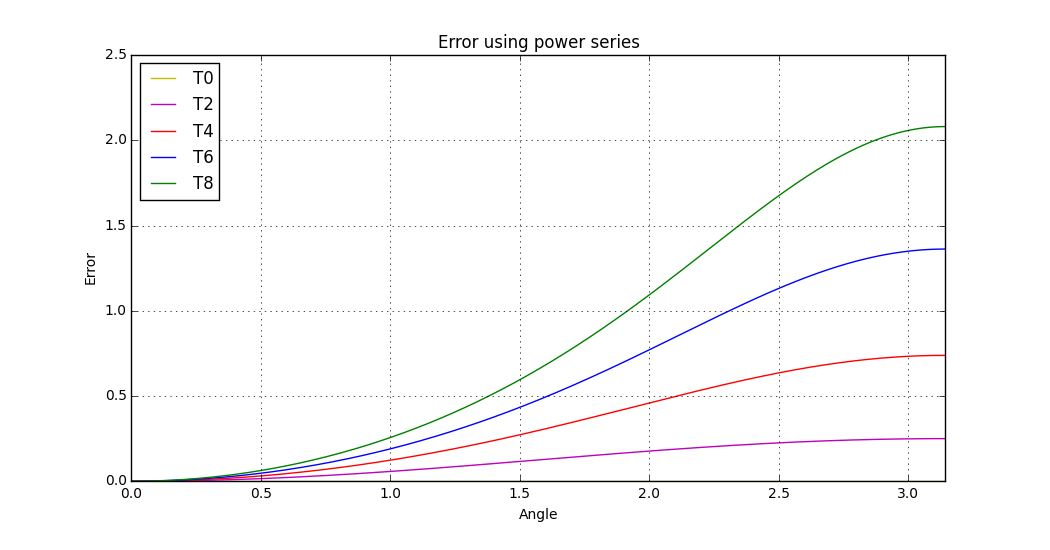
\includegraphics[width=12cm]{p.png}
	\caption{Resultados}
\end{figure}

\begin{thebibliography}{6}
	
	\bibitem{P}
	\emph{Maxima}. 
	\url{http://maxima.sourceforge.net/es/}
	

	\bibitem{U}
	\emph{Péndulo}
	\url{https://en.wikipedia.org/wiki/Pendulum_%28mathematics%29}
	
\end{thebibliography}



\end{document}

